\section{Casi d'uso} \label{section:casi_uso}

\subsection{Scopo}
Lo scopo di questa sezione è la descrizione in elenco di tutti i casi d'uso individuati dal gruppo, in
riferimento alle funzionalità dell'applicazione.

\subsection{Attori}
Come accordato con il proponente, la web app\glo{} deve essere usata sia dal venditore che dal cliente,
sono quindi presenti tre attori nella gerarchia: la piattaforma e-commerce\glo{} da cui parte l'ordine, Metamask\glo{}, l'utente generico.
L'utente generico ha poi due specializzazioni possibili: l'utente proprietario dell'ordine e l'utente venditore.

\begin{figure}[H]
    \centering
    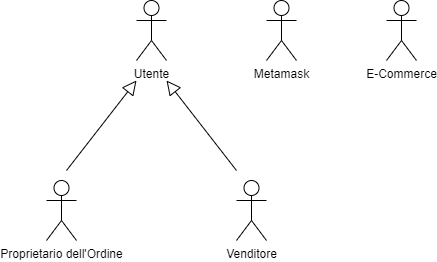
\includegraphics[scale=0.7]{immagini/UseCases-Attori.png}
    \caption{Diagramma degli attori}
\end{figure}

\subsection{UC1 - Inizializzazione della Transazione}\label{subsection: UC1}

\begin{figure}[H]
    \centering
    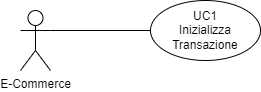
\includegraphics[scale=0.7]{immagini/UseCases-UC1.png}
    \caption{UC1}
\end{figure}

\begin{itemize}
    \item Attore primario: e-commerce\glo{};
    \item Precondizioni: il sistema è raggiungibile e funzionante;
    \item Postcondizioni: la transazione viene caricata nel sistema, l'utente viene reindirizzato alla pagina di checkout;
    \item Scenario principale: L'e-commerce\glo{} delega il pagamento comunicando la somma richiesta e l'indirizzo del destinatario.
\end{itemize}

\subsection{UC2 - Checkout}\label{subsection: UC2}

\begin{figure}[H]
    \centering
    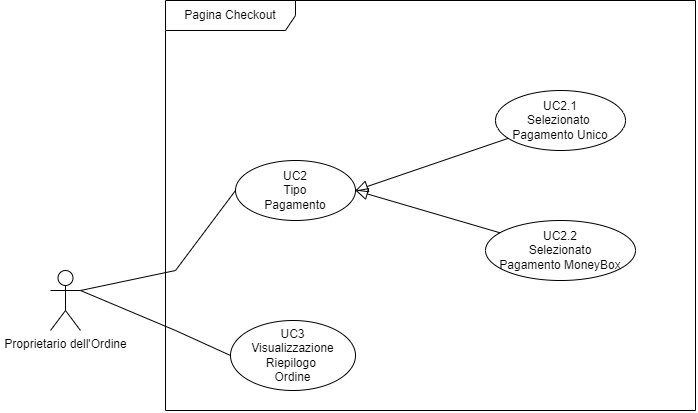
\includegraphics[scale=0.7]{immagini/UseCases-UC2-1.png}
    \caption{Pagina di checkout}
\end{figure}

\begin{itemize}
    \item Attore primario: Utente proprietario dell'ordine, utente generico;
    \item Precondizioni: l'e-commerce\glo{} ha iniziato la transazione [UC1];
    \item Postcondizioni: viene visualizzato l'esito dell'operazione;
    \item Scenario principale:
    \begin{enumerate}
        \item L'utente visualizza il riepilogo dell'ordine [UC2.1];
        \item L'utente seleziona la tipologia di pagamento tra quelle disponibili [UC2.2];
        \item L'utente effettua il pagamento [UC2.3].
    \end{enumerate}
\end{itemize}

\subsubsection{UC2.1 - Visualizzazione Riepilogo Ordine}\label{sssec: UC2.1}

\begin{itemize}
    \item Attore primario: utente generico;
    \item Precondizioni: l'e-commerce\glo{} ha iniziato la transazione [UC1];
    \item Postcondizioni: l'utente ha visualizzato il riepilogo dell'ordine;
    \item Scenario principale:
          \begin{enumerate}
              \item L'utente visualizza il totale dell'ordine;
              \item L'utente visualizza l'indirizzo del venditore.
          \end{enumerate}
\end{itemize}

\subsubsection{UC2.2 - Selezione Tipo Pagamento}\label{sssec: UC2.2}

\begin{itemize}
    \item Attore primario: utente proprietario dell'ordine;
    \item Precondizioni: l'e-commerce\glo{} ha iniziato la transazione [UC1];
    \item Postcondizioni: l'utente ha selezionato un metodo di pagamento;
    \item Scenario principale: Se la transazione non risulta registrata in blockchain, l'utente seleziona la tipologia di pagamento.
    \item Estensioni:
          \begin{enumerate}
            \item Nel caso in cui la transazione interessata sia presente in blockchain:
                \begin{itemize}
                    \item La selezione della tipologia di pagamento viene omessa;
                    \item Viene visualizzato Avviso Transazione Esistente [UC2.2.3].
                \end{itemize}
          \end{enumerate}
\end{itemize}

\paragraph{UC2.2.1 - Selezionato Pagamento Unico}\label{sssec: UC2.2.1}

\begin{itemize}
    \item Attore primario: utente proprietario dell'ordine;
    \item Precondizioni: l'e-commerce\glo{} ha iniziato la transazione [UC1];
    \item Postcondizioni: l'utente ha selezionato pagamento unico come metodo di pagamento;
    \item Scenario principale: L'utente seleziona pagamento unico come metodo di pagamento.
\end{itemize}

\paragraph{UC2.2.2 -  Selezionato Pagamento MoneyBox}

\begin{itemize}
    \item Attore primario: utente proprietario dell'ordine;
    \item Precondizioni: l'e-commerce\glo{} ha iniziato la transazione [UC1];
    \item Postcondizioni: l'utente ha selezionato pagamento MoneyBox\glo{} come metodo di pagamento;
    \item Scenario principale: L'utente seleziona pagamento MoneyBox\glo{} come metodo di pagamento.
\end{itemize}

\paragraph{UC2.2.3 - Visualizzazione avviso transazione esistente}

\begin{itemize}
    \item Attore primario: utente proprietario dell'ordine;
    \item Precondizioni: l'e-commerce\glo{} ha iniziato la transazione [UC1];
    \item Postcondizioni: l'utente visualizza il messaggio di avviso transazione esistente;
    \item Scenario principale: l'utente visualizza il messaggio di avviso, poichè la transazione è già presente in blockchain.
\end{itemize}

\subsubsection{UC2.3 - Pagamento}

\begin{figure}[H]
    \centering
    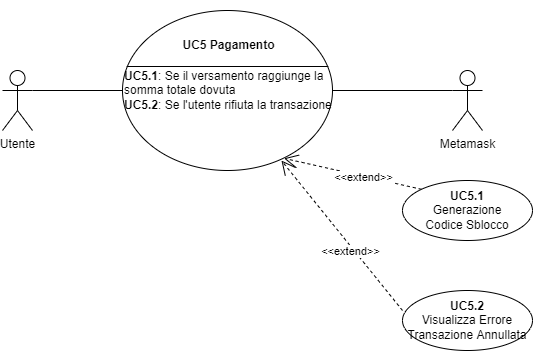
\includegraphics[scale=0.7]{immagini/UseCases-UC5.png}
    \caption{UC2.3}
\end{figure}

\begin{itemize}
    \item Attore primario: utente generico;
    \item Attore secondario: Metamask\glo{};
    \item Precondizioni: è stata selezionata una tipologia di pagamento per la transazione interessata [UC2.2], l'utente ha connesso il proprio wallet\glo{} tramite Metamask\glo{} [UC4];
    \item Postcondizioni: l'utente ha effettuato il pagamento;
    \item Scenario principale:
          \begin{enumerate}
              \item L'utente visualizza il pop-up di Metamask\glo{} con i dettagli della transazione;
              \item L'utente visualizza un overlay di caricamento sulla pagina di ShopChain;
              \item L'utente autorizza la transazione per l'importo impostato;
              \item L'utente visualizza un messaggio di conferma di avvenuto pagamento.
          \end{enumerate}
    \item Estensioni:
          \begin{enumerate}
              \item Nel caso venisse raggiunta la somma totale dovuta, viene generato e mostrato il codice di sblocco [UC2.3.3];
              \item Nel caso l'utente rifiuti il pagamento:
              \begin{itemize}
                  \item La transazione viene annullata;
                  \item L'utente visualizza errore transazione annullata [UC2.3.4].
              \end{itemize}
          \end{enumerate}
    \item Generalizzazioni:
          \begin{enumerate}
              \item Pagamento Unico [UC2.3.1];
              \item Pagamento MoneyBox [UC2.3.2].
          \end{enumerate}
\end{itemize}

\paragraph{UC2.3.1 - Pagamento Unico}

\begin{itemize}
    \item Attore primario: utente proprietario dell'ordine;
    \item Precondizioni: è stata selezionato Pagamento Unico come tipologia di pagamento per la transazione interessata [UC2.2.1], l'utente ha connesso il proprio wallet\glo{} tramite Metamask\glo{} [UC4];
    \item Postcondizioni: l'utente ha pagato l'importo totale in un pagamento unico;
    \item Scenario principale:
    \begin{enumerate}
        \item L'utente visualizza il pop-up di Metamask\glo{} con i dettagli della transazione;
        \item L'utente visualizza un overlay di caricamento sulla pagina di ShopChain;
        \item L'utente autorizza la transazione per un pagamento unico corrispondente all'importo totale;
        \item L'utente visualizza un messaggio di conferma di avvenuto pagamento.
    \end{enumerate}
\end{itemize}

\paragraph{UC2.3.2 - Pagamento MoneyBox}

\begin{itemize}
    \item Attore primario: utente generico;
    \item Precondizioni: è stata selezionato Pagamento MoneyBox\glo{} come tipologia di pagamento per la transazione interessata [UC2.2.2], l'utente ha connesso il proprio wallet\glo{} tramite Metamask\glo{} [UC4];
    \item Postcondizioni: l'utente ha pagato l'importo scelto;
    \item Scenario principale:
    \begin{enumerate}
        \item L'utente visualizza il pop-up di Metamask\glo{} con i dettagli della transazione;
        \item L'utente visualizza un overlay di caricamento sulla pagina di ShopChain;
        \item L'utente autorizza la transazione per l'importo scelto;
        \item L'utente visualizza un messaggio di conferma di avvenuto pagamento.
    \end{enumerate}
\end{itemize}

\paragraph{UC2.3.3 - Generazione Codice di Sblocco}

\begin{itemize}
    \item Attore primario: utente generico;
    \item Precondizioni: il versamento raggiunge la somma totale dovuta;
    \item Postcondizioni: l'utente ha visualizzato il codice di sblocco;
    \item Scenario principale:
          \begin{enumerate}
              \item Viene generato il codice di sblocco;
              \item L'utente visualizza il codice di sblocco.
          \end{enumerate}
\end{itemize}

\paragraph{UC2.3.4 - Visualizzazione errore transazione annullata}

\begin{itemize}
    \item Attore primario: utente generico;
    \item Precondizioni: la transazione non è andata a buon fine;
    \item Postcondizioni: l'utente ha visualizzato l'errore e la transazione fallisce;
    \item Scenario principale:
          \begin{enumerate}
              \item L'utente visualizza un messaggio di errore per rifiuto della transazione;
              \item L'utente clicca ”OK” per continuare.
          \end{enumerate}
\end{itemize}

\subsection{UC3 - Gestione MoneyBox}

\begin{figure}[H]
    \centering
    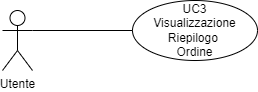
\includegraphics[scale=0.7]{immagini/UseCases-UC3.png}
    \caption{UC3}
\end{figure}

\begin{itemize}
    \item Attore primario: utente generico;
    \item Precondizioni: l'e-commerce\glo{} ha iniziato la transazione [UC1], l'utente dispone dell'invito valido ad una MoneyBox\glo{};
    \item Postcondizioni: l'utente ha visualizzato i dati relativi la MoneyBox;
    \item Scenario principale:
          \begin{enumerate}
                \item L'utente può visualizzare lo stato del completamento in formato percentuale e il saldo mancante [UC3.1];
                \item L'utente può visualizzare un elenco delle transazioni partecipanti [UC3.2];
                \item L'utente può visualizzare l'invito per partecipare alla MoneyBox [UC3.3];
                \item L'utente può partecipare alla MoneyBox [UC3.4];
                \item L'utente può visualizzare una grafica identificativa della MoneyBox [UC3.5].
    \end{enumerate}
\end{itemize}

\subsubsection{UC3.1 - Visualizzazione Stato Completamento}

\begin{itemize}
    \item Attore primario: utente generico;
    \item Precondizioni: l'e-commerce\glo{} ha iniziato la transazione [UC1], l'utente dispone dell'invito valido ad una MoneyBox\glo{};
    \item Postcondizioni: l'utente ha visualizzato lo stato del completamento;
    \item Scenario principale:
          \begin{enumerate}
              \item L'utente visualizza lo stato del completamento in formato percentuale e il saldo mancante;
              \item L'utente visualizza un elenco delle transazioni partecipanti [UC3.2].
          \end{enumerate}
\end{itemize}

\subsubsection{UC3.2 - Visualizzazione Elenco Transazioni Partecipanti}

\begin{itemize}
    \item Attore primario: utente generico;
    \item Precondizioni: l'e-commerce\glo{} ha iniziato la transazione [UC1], l'utente dispone dell'invito valido ad una MoneyBox\glo{};
    \item Postcondizioni: l'utente ha visualizzato l'invito alla MoneyBox\glo{};
    \item Scenario principale: l'utente visualizza l'invito alla MoneyBox\glo{}.
\end{itemize}

\subsubsection{UC3.3 - Visualizzazione Invito Partecipazione MoneyBox}

\begin{itemize}
    \item Attore primario: utente generico;
    \item Precondizioni: l'e-commerce\glo{} ha iniziato la transazione [UC1], l'utente dispone dell'invito valido ad una MoneyBox\glo{};
    \item Postcondizioni: l'utente ha visualizzato l'invito alla MoneyBox\glo{};
    \item Scenario principale: l'utente visualizza l'invito alla MoneyBox\glo{}.
\end{itemize}

\subsubsection{UC3.4 - Partecipazione MoneyBox}

\begin{itemize}
    \item Attore primario: utente generico;
    \item Precondizioni: l'e-commerce\glo{} ha iniziato la transazione [UC1], l'utente dispone dell'invito valido ad una MoneyBox\glo{};
    \item Postcondizioni: l'utente ha selezionato la quota da versare e ha effettuato il pagamento;
    \item Scenario principale:
          \begin{enumerate}
              \item L'utente seleziona la quota da versare, compresa tra zero escluso e il minimo tra il saldo disponibile nel wallet e il rimanente della MoneyBox\glo{};
              \item L'utente effettua il pagamento [UC5].
          \end{enumerate}
\end{itemize}

\subsubsection{UC3.5 - Visualizzazione Grafica Identificativa}

\begin{itemize}
    \item Attore primario: utente generico;
    \item Precondizioni: 
    \item Postcondizioni: 
    \item Scenario principale:
\end{itemize}

\subsection{UC4 - Connessione Metamask}

\begin{figure}[H]
    \centering
    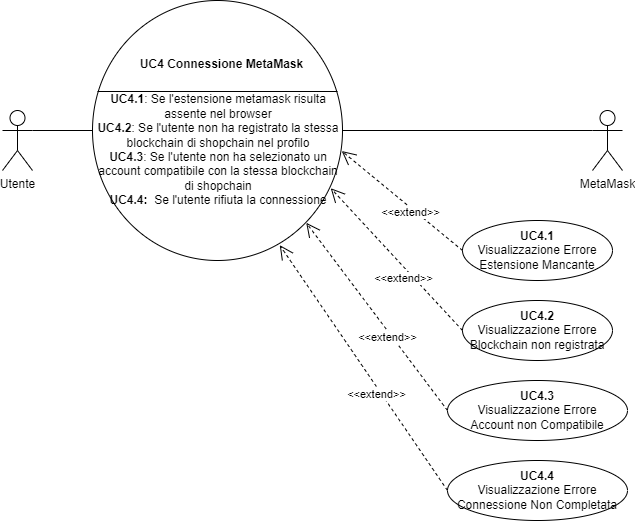
\includegraphics[scale=0.7]{immagini/UseCases-UC4.png}
    \caption{UC4}
\end{figure}

\begin{itemize}
    \item Attore primario: utente generico;
    \item Precondizioni: il sistema è raggiungibile e funzionante;
    \item Postcondizioni: l'utente ha connesso Metamask\glo{} a ShopChain;
    \item Scenario principale:
        \begin{enumerate}
            \item L'utente visualizza il pop-up di Metamask\glo{} per la connessione a ShopChain;
            \item L'utente autorizza la connessione a ShopChain.
        \end{enumerate}
    \item Estensioni:
        \begin{enumerate}
            \item Nel caso in cui l'estensione Metamask\glo{} risultasse assente nel browser:
                \begin{itemize}
                    \item La connessione non ha successo;
                    \item Viene visualizzato errore estensione mancante [UC4.1].
                \end{itemize}
            \item Nel caso in cui l'utente abbia connesso il proprio wallet\glo{} ma non abbia configurato la stessa blockchain\glo{} di ShopChain:
                \begin{itemize}
                    \item La connessione non viene completata;
                    \item Viene visualizzato errore blockchain\glo{} non registrata [UC4.2].
                \end{itemize}
            \item Nel caso in cui l'utente abbia configurato la stessa blockchain\glo{} di ShopChain ma non selezionato un account compatibile:
                \begin{itemize}
                    \item La connessione non viene completata;
                    \item Viene visualizzato errore account non compatibile [UC4.3].
                \end{itemize}
            \item Nel caso l'utente rifiuti la connessione, visualizza errore connessione non completata [UC4.4].
        \end{enumerate}
\end{itemize}

\subsubsection{UC4.1 - Visualizzazione Errore Estensione Mancante}

\begin{itemize}
    \item Attore primario: utente generico;
    \item Precondizioni: l'utente utilizza un browser sprovvisto di estensione Metamask\glo{};
    \item Postcondizioni: l'utente ha visualizzato l'errore e la connessione fallisce;
    \item Scenario principale:
        \begin{enumerate}
            \item L'utente visualizza un messaggio di errore per mancata connessione;
            \item L'utente viene invitato a scaricare l'estensione Metamask\glo{};
            \item L'utente clicca ”OK” per continuare.
        \end{enumerate}
\end{itemize}

\subsubsection{UC4.2 - Visualizzazione Errore Blockchain non registrata}

\begin{itemize}
    \item Attore primario: utente generico;
    \item Precondizioni: l'utente ha connesso il proprio wallet\glo{} ma non ha configurato la stessa blockchain\glo{} di ShopChain;
    \item Postcondizioni: l'utente ha visualizzato l'errore e la connessione fallisce;
    \item Scenario principale:
          \begin{enumerate}
              \item L'utente visualizza un messaggio di errore per mancata connessione;
              \item L'utente visualizza i dati per configurare la blockchain\glo{};
              \item L'utente clicca ”OK” per continuare.
          \end{enumerate}
\end{itemize}

\subsubsection{UC4.3 - Visualizzazione Errore account non compatibile}

\begin{itemize}
    \item Attore primario: utente generico;
    \item Precondizioni: l'utente ha configurato la stessa blockchain\glo{} di ShopChain ma non ha selezionato un account compatibile;
    \item Postcondizioni: l'utente ha visualizzato l'errore e la connessione fallisce;
    \item Scenario principale:
          \begin{enumerate}
              \item L'utente visualizza un messaggio di errore per mancata connessione;
              \item L'utente viene invitato a cambiare account o a registrare un account compatibile;
              \item L'utente clicca ”OK” per continuare.
          \end{enumerate}
\end{itemize}

\subsubsection{UC4.4 - Visualizzazione Errore connessione non completata}

\begin{itemize}
    \item Attore primario: utente generico;
    \item Precondizioni: l'utente rifiuta la connessione;
    \item Postcondizioni: l'utente ha visualizzato l'errore e la connessione fallisce;
    \item Scenario principale:
          \begin{enumerate}
              \item L'utente visualizza un messaggio di errore per mancata connessione;
              \item L'utente viene invitato a ritentare;
              \item L'utente clicca ”OK” per continuare.
          \end{enumerate}
\end{itemize}

\subsection{UC5 - Visualizzazione Indirizzo Wallet}

\begin{figure}[H]
    \centering
    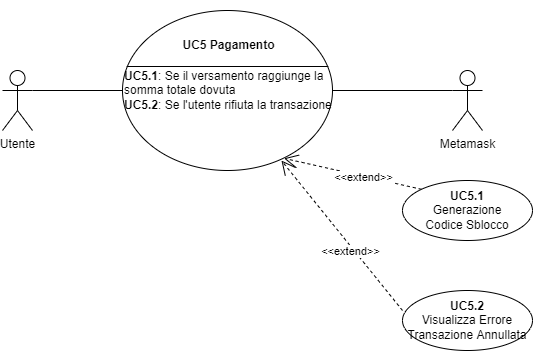
\includegraphics[scale=0.7]{immagini/UseCases-UC5.png}
    \caption{UC5}
\end{figure}

\begin{itemize}
    \item Attore primario: utente generico;
    \item Precondizioni: il sistema è raggiungibile e funzionante;
    \item Postcondizioni: l'utente ha visualizzato l'indirizzo del wallet;
    \item Scenario principale: l'utente visualizza l'indirizzo del wallet.
    \item Estensioni:
    \begin{enumerate}
        \item Visualizzazione Avviso Connessione Metamask [UC5.3].
    \end{enumerate}
    \item Generalizzazioni:
    \begin{enumerate}
        \item Visualizzazione Indirizzo Wallet Testuale [UC5.1];
        \item Visualizzazione Indirizzo Wallet Emoji [UC5.2].
    \end{enumerate}
\end{itemize}

\subsubsection{UC5.1 - Visualizzazione Indirizzo Wallet Testuale}

\begin{itemize}
    \item Attore primario: utente generico;
    \item Precondizioni: il sistema è raggiungibile e funzionante;
    \item Postcondizioni: l'utente ha visualizzato l'indirizzo del wallet in forma testuale;
    \item Scenario principale: l'utente visualizza l'indirizzo del wallet in forma testuale.
\end{itemize}

\subsubsection{UC5.2 - Visualizzazione Indirizzo Wallet Emoji}

\begin{itemize}
    \item Attore primario: utente generico;
    \item Precondizioni: il sistema è raggiungibile e funzionante;
    \item Postcondizioni: l'utente ha visualizzato l'indirizzo del wallet sotto forma di sequenza di emoji;
    \item Scenario principale: l'utente visualizza l'indirizzo del wallet sotto forma di sequenza di emoji.
\end{itemize}

\subsubsection{UC5.3 - Visualizzazione Avviso Connessione Metamask}

\begin{itemize}
    \item Attore primario: utente generico;
    \item Precondizioni: l'utente non ha effettuato la connessione a Metamask;
    \item Postcondizioni: l'utente ha visualizzato un avviso relativo la mancata connessione a Metamask;
    \item Scenario principale: l'utente visualizza un avviso relativo la mancata connessione a Metamask.
\end{itemize}

\subsubsection{UC6 - Sblocco Ordine}

\begin{figure}[H]
    \centering
    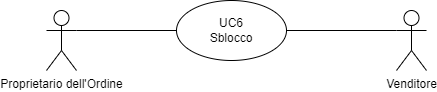
\includegraphics[scale=0.7]{immagini/UseCases-UC6.png}
    \caption{Pagina transazione pagata}
\end{figure}

\begin{itemize}
    \item Attore primario: utente proprietario dell'ordine;
    \item Attore secondario: utente venditore, Metamask\glo{};
    \item Precondizioni: il sistema ha generato il codice di sblocco [UC2.3.3];
    \item Postcondizioni: l'utente proprietario ha sbloccato l'ordine e il denaro è stato trasferito all'utente venditore;
    \item Scenario principale:
          \begin{enumerate}
              \item L'utente inserisce il codice di sblocco;
              \item L'utente conferma la transazione sul pop-up Metamask\glo{};
              \item Il sistema trasferisce il denaro sul wallet\glo{} dell'utente venditore.
          \end{enumerate}
\end{itemize}

\subsection{UC7 - Visualizzazione Transazioni}

\begin{figure}[H]
    \centering
    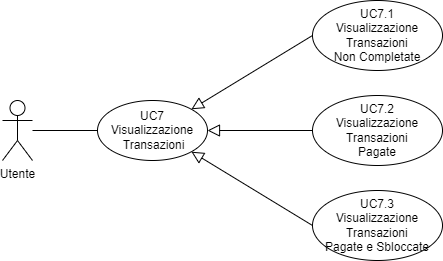
\includegraphics[scale=0.7]{immagini/UseCases-UC7.png}
    \caption{UC7 e i suoi sottocasi}
\end{figure}

\begin{itemize}
    \item Attore primario: utente generico;
    \item Precondizioni: il sistema è raggiungibile e funzionante;
    \item Postcondizioni: l'utente ha selezionato il tipo delle transazioni che vuole visualizzare;
    \item Scenario principale: l'utente sceglie il tipo delle transazioni da visualizzare tra quelli disponibili;
    \item Generalizzazioni: l'utente sceglie una delle seguenti opzioni:
          \begin{itemize}
              \item Visualizza transazioni in entrata [UC7.1];
              \item Visualizza transazioni in uscita [UC7.2];
          \end{itemize}
\end{itemize}

\subsubsection{UC7.1 - Visualizza Transazioni In Entrata Pagate}

\begin{itemize}
    \item Attore primario: utente generico;
    \item Precondizioni: l'utente ha selezionato le transazioni in entrata;
    \item Postcondizioni: l'utente ha visualizzato le transazioni in entrata;
    \item Scenario principale: l'utente sceglie le transazioni in entrata per essere visualizzate;
    \item Generalizzazioni: l'utente sceglie una delle seguenti opzioni:
          \begin{itemize}
              \item Visualizza transazioni non sbloccate [UC7.1.1];
              \item Visualizza transazioni sbloccate [UC7.1.2];
              \item Visualizza transazioni cancellate [UC7.1.3].
          \end{itemize}
\end{itemize}

\paragraph{UC7.1.1 - Visualizza Transazioni Non Sbloccate}

\begin{itemize}
    \item Attore primario: utente generico;
    \item Precondizioni: l'utente ha selezionato visualizza transazioni non sbloccate;
    \item Postcondizioni: l'utente ha visualizzato la lista di transazioni non sbloccate;
    \item Scenario principale: l'utente visualizza la lista di transazioni non sbloccate.
\end{itemize}

\paragraph{UC7.1.2 - Visualizza Transazioni Sbloccate}

\begin{itemize}
    \item Attore primario: utente generico;
    \item Precondizioni: l'utente ha selezionato visualizza transazioni sbloccate;
    \item Postcondizioni: l'utente ha visualizzato la lista di transazioni sbloccate;
    \item Scenario principale: l'utente visualizza la lista di transazioni sbloccate.
\end{itemize}

\paragraph{UC7.1.3 - Visualizza Transazioni Cancellate}

\begin{itemize}
    \item Attore primario: utente generico;
    \item Precondizioni: l'utente ha selezionato visualizza transazioni cancellate;
    \item Postcondizioni: l'utente ha visualizzato la lista di transazioni cancellate;
    \item Scenario principale: l'utente visualizza la lista di transazioni cancellate.
\end{itemize}

\subsubsection{UC7.2 - Visualizza Transazioni In Uscita}

\begin{itemize}
    \item Attore primario: utente proprietario dell'ordine;
    \item Precondizioni: l'utente ha selezionato le transazioni in uscita;
    \item Postcondizioni: l'utente ha visualizzato le transazioni in uscita;
    \item Scenario principale: l'utente sceglie le transazioni in uscita per essere visualizzate;
    \item Generalizzazioni: l'utente sceglie una delle seguenti opzioni:
          \begin{itemize}
              \item Visualizza transazioni non pagate [UC7.2.1];
              \item Visualizza transazioni pagate ma non sbloccate [UC7.2.2];
              \item Visualizza transazioni pagate e sbloccate [UC7.2.3].
          \end{itemize}
\end{itemize}

\paragraph{UC7.2.1 - Visualizza Transazioni Non Pagate}

\begin{itemize}
    \item Attore primario: utente proprietario dell'ordine;
    \item Precondizioni: l'utente ha selezionato visualizza transazioni non pagate;
    \item Postcondizioni: l'utente ha visualizzato la lista di transazioni non pagate;
    \item Scenario principale: l'utente visualizza la lista di transazioni non pagate.
\end{itemize}

\paragraph{UC7.2.2 - Visualizza Transazioni Pagate Ma Non Sbloccate}

\begin{itemize}
    \item Attore primario: utente proprietario dell'ordine;
    \item Precondizioni: l'utente ha selezionato visualizza transazioni pagate ma non sbloccate;
    \item Postcondizioni: l'utente ha visualizzato la lista di transazioni pagate pagate ma non sbloccate;
    \item Scenario principale: l'utente visualizza la lista di transazioni pagate pagate ma non sbloccate.
\end{itemize}

\paragraph{UC7.2.3 - Visualizza Transazioni Pagate e Sbloccate}

\begin{itemize}
    \item Attore primario: utente proprietario dell'ordine;
    \item Precondizioni: l'utente ha selezionato visualizza transazioni pagate e sbloccate;
    \item Postcondizioni: l'utente ha visualizzato la lista di transazioni pagate e sbloccate;
    \item Scenario principale: l'utente visualizza la lista di transazioni pagate e sbloccate.
\end{itemize}

\paragraph{UC7.2.4 - Visualizza Transazioni Cancellate}

\begin{itemize}
    \item Attore primario: utente proprietario dell'ordine;
    \item Precondizioni: l'utente ha selezionato visualizza transazioni cancellate;
    \item Postcondizioni: l'utente ha visualizzato la lista di transazioni cancellate;
    \item Scenario principale: l'utente visualizza la lista di transazioni cancellate.
\end{itemize}

\subsection{UC8 - Rimborso}

\begin{itemize}
    \item Attore primario: utente proprietario dell'ordine, utente venditore;
    \item Attore secondario: Metamask\glo{};
    \item Precondizioni: l'utente ha connesso il proprio Metamask\glo{} [UC4] ed esiste almeno un pagamento associato all'indirizzo dell'utente;
    \item Postcondizioni: l'utente ha annullato l'ordine e i fondi vengono restituiti;
    \item Scenario principale:
          \begin{enumerate}
              \item L'utente visualizza il pop-up di Metamask\glo{};
              \item L'utente conferma l'operazione all'interno del pop-up;
              \item Viene annullato ogni versamento ed effettuati i rimborsi.
          \end{enumerate}
\end{itemize}

\clearpage
